\documentclass[article]{jss}
\usepackage[utf8]{inputenc}

\providecommand{\tightlist}{%
  \setlength{\itemsep}{0pt}\setlength{\parskip}{0pt}}

\author{
Anna Michalek\\European Central Bank \And Alain Quartier-la-Tente\\Insee
}
\title{\pkg{RJDemetra}: A R Interface To JDemetra+ Seasonal Adjustment Software}

\Plainauthor{Anna Michalek, Alain Quartier-la-Tente}
\Plaintitle{A Capitalized Title: Something about a Package foo}
\Shorttitle{\pkg{RJDemetra}: A R Interface To JDemetra+ Seasonal Adjustment Software}

\Abstract{
The abstract of the article.
}

\Keywords{\proglang{R}, seasonal adjustment, calendar effects, time series}
\Plainkeywords{R, seasonal adjustment, calendar effects, time series}

%% publication information
%% \Volume{50}
%% \Issue{9}
%% \Month{June}
%% \Year{2012}
%% \Submitdate{}
%% \Acceptdate{2012-06-04}

\Address{
    }

% Pandoc header

\usepackage{amsmath} \usepackage{booktabs} \usepackage{longtable} \usepackage{array} \usepackage{multirow} \usepackage{wrapfig} \usepackage{float} \usepackage{pdflscape} \usepackage{tabu} \usepackage{threeparttable} \usepackage{threeparttablex} \usepackage[normalem]{ulem} \usepackage{makecell}

\begin{document}

\hypertarget{introduction}{%
\section{Introduction}\label{introduction}}

Since the 20th century, more and more infra-annual statistics are
produced, especially by national institutes, to analyse the progression
and the outlook of an economy. It is for example the case of the gross
domestic product (GDP), unemployment rate, household consumption of
goods and industrial production indices. However, most of those time
series are affected by seasonal and trading day effects. A seasonal
effects is an effect that occur in the same calendar month with similar
magnitude and direction from year to year. For instance, automobile
production is usually lower during summer, due to holidays, and
chocolate sales are usually higher in December, due to Christmas.
Trading day effect is the fact that a time series can be affected by
each calendar month's weekday composition. For example retail sales are
usually higher on Saturday, thus they are likely to be higher in months
with a surplus of weekend days.

Therefore, seasonal and trading days effects can make it difficult to
analyse the infra-annual movements of a time series or to make spatial
comparison. That's why time series are often seasonally and working day
adjusted and seasonal adjustment is the process of removing the effects
of seasonal and trading day fluctuations.

The most popular seasonal adjustment methods are TRAMO-SEATS+\footnote{The
  program TRAMO-SEATS+ was developed by Gianluca Caporello and Agustin
  Maravall --- with programming support from Domingo Perez and Roberto
  Lopez --- at the Bank of Spain. It is based on the program
  TRAMO-SEATS, previously developed by Victor Gomez and Agustin
  Maravall.} \citep{gomez1996programs, caporello2004program}, a
parametric method based on ARIMA models, and X-13-ARIMA-SEATS\footnote{The
  program X-13ARIMA-SEATS is a produced, distributed, and maintained by
  the US-Census Bureau.} \citep{findleyx12, ladiray1999x11en}, a
non-parametric method based on moving average. Both methods are
recommended by Eurostat and the European Central Bank (ECB) to
seasonnaly adjust economic indicators. These methods proceed in two
steps summarized in figure \ref{fig:2_step_proc}.

\begin{figure}[htb]
\centering
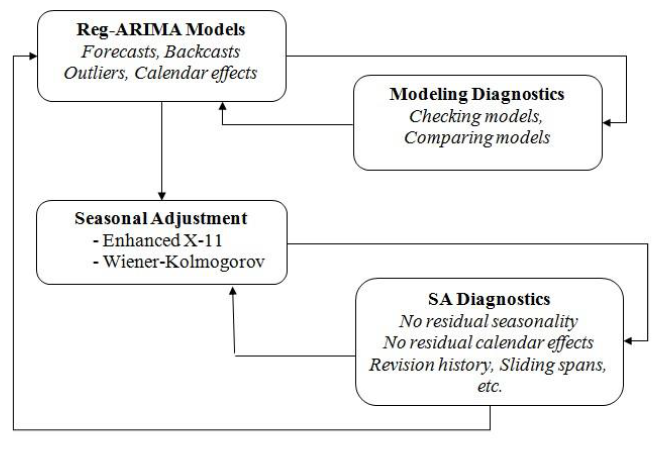
\includegraphics[scale=0.8]{img/sa_2_steps.PNG} 
\caption{X-13-ARIMA-SEATS and TRAMO-SEATS+ 2-step process: pre-adjustment and decomposition.}
\label{fig:2_step_proc}
\end{figure}

The \textbf{first step} of seasonal adjustment consists of pre-adjusting
the time series by removing from it the deterministic effects and
estimating missing observations. Among deterministic effects, we
distinguish outliers, calendar and regression effects. In this step,
also forecasts and backcasts of the pre-adjusted series are estimated
which allows applying linear filters at both ends of the series in the
second step of the seasonal adjustment. The pre-adjustment,
linearization, of the input series is achieved with a \textbf{RegARIMA}
model (model with ARIMA errors) as specified below.

\[z_t=y_t\beta+x_t\] where

\begin{itemize}
\tightlist
\item
  \(z_t\) - is the original series;
\item
  \(\beta = (\beta_1,...,\beta_n)\) - a vector of regression
  coefficients;
\item
  \(y_t = (y_{1t},...,y_{nt})\) - \(n\) regression variables (outliers,
  calendar effects, user-defined variables);
\item
  \(x_t\) - a disturbance that follows the general ARIMA process:
\item
  \(\phi(B)\delta(B)x_t=\theta(B)a_t\); \(\phi(B), \delta(B)\) and
  \(\theta(B)\) are the finite polynomials in \(B\); \(a_t\) is a
  white-noise variable with zero mean and a constant variance.
\end{itemize}

The polynomial \(\phi(B)\) is a stationary autoregressive (AR)
polynomial in \(B\), which is a product of the stationary regular AR
polynomial in \(B\) and the stationary seasonal polynomial in \(B^s\):

\[\phi(B)=\phi_p(B)\Phi_{bp}(B^s)=(1+\phi_1B+...+\phi_pB^p)(1+\Phi_1B^s+...+\Phi_{bp}B^{bps}\]

where:

\begin{itemize}
\tightlist
\item
  \(p\) - number of regular AR terms (in the package and in JDemetra+
  \(p \le 3\));
\item
  \(bp\) - number of seasonal AR terms (in the package and in JDemetra+
  \(bp \le 1\));
\item
  \(s\) - number of observations per year (frequency of the time
  series).
\end{itemize}

The polynomial \(\theta(B)\) is an invertible moving average (MA)
polynomial in \(B\), which is a product of the invertible regular MA
polynomial in \(B\) and the invertible seasonal MA polynomial in
\(B^s\):

\[\theta(B)=\theta_q(B)\Theta_{bq}(B^s)=(1+\theta_1B+...+\theta_qB^q)(1+\Theta_1B^s+...+\Theta_{bq}B^{bqs})\]

where:

\begin{itemize}
\tightlist
\item
  \(q\) - number of regular MA terms (in the package and in JDemetra+
  \(q \le 3\));
\item
  \(bq\) - number of seasonal MA terms (in the package and in JDemetra+
  \(bq \le 1\));
\end{itemize}

The polynomial \(\delta(B)\) is the non-stationary AR polynomial in
\(B\) (unit roots):

\[\delta(B)=(1-B)^d(1-B^s)^{d_s}\]

where:

\begin{itemize}
\tightlist
\item
  \(d\) - regular differencing order (in the package and in JDemetra+
  \(d \le 1\));
\item
  \(d_s\) - seasonal differencing order (in the package and in JDemetra+
  \(d_s \le 1\));
\end{itemize}

An automatic modelling is also implemented in both methods to: determine
the decomposition of the series, detect outliers and calendar effects
and to adjust residuals to an ARIMA models. A detailed description can
be found in \cite{gomez1998automatic}.

In the \textbf{second part} of seasonal adjustment, called the
\textbf{decomposition}, the pre-adjusted series (\(y\)) is decomposed
into the following components: trend-cycle (\(t\)), seasonal component
(\(s\)) and irregular component (\(i\)). The decomposition can be:

\begin{itemize}
\tightlist
\item
  additive (\(y = t + s + i\))\\
\item
  multiplicative (\(y = t * s * i\))\\
\item
  log-additive (\(\log(y) = \log(t) + \log(s) + \log(i)\)) or\\
\item
  pseudo-additive (\(y = t * (s + i - 1)\))
\end{itemize}

The last two decompositions are available only under X13 (? à discuter).

The method of decomposing the pre-adjusted series differs between
TRAMO-SEATS+ and X-12ARIMA/X-13ARIMA. In TRAMO-SEATS+, SEATS (Signal
Extraction in ARIMA Time Series) decomposes the observed series with a
ARIMA-model based method
\citep{gomez1996programs, caporello2004program}. Whereas in
X-12ARIMA/X-13ARIMA, the X-11 algorithm decomposes the time series by
means of linear filters \citep{findleyx12, ladiray1999x11en}.

As a result of seasonal adjustment, the final seasonally adjusted series
shall be free of seasonal and calendar-related movements.

\hypertarget{jdemetra-and-rjdemetra}{%
\section{JDemetra+ and RJDemetra}\label{jdemetra-and-rjdemetra}}

JDemetra+ is a new tool for seasonal adjustment (SA) developed by the
National Bank of Belgium (NBB) in cooperation with the Deutsche
Bundesbank and Eurostat in accordance with the Guidelines of the
European Statistical System (ESS) \citep{eurostat2015guidelines}. It
implements the concepts and algorithms used in the two leading SA
methods: TRAMO-SEATS+ and X-12ARIMA/X-13ARIMA-SEATS. Those methods have
been re-engineered using an object-oriented approach that enables easier
handling, extensions and modifications.

JDemetra+ has been
\href{https://ec.europa.eu/eurostat/cros/system/files/Jdemetra_\%20release.pdf}{officially
recommended}, since 2 February 2015, to the members of the ESS and the
European System of Central Banks as software for seasonal and calendar
adjustment of official statistics.

Besides seasonal adjustment, JDemetra+ bundles other time series models
that are useful in the production or analysis of economic statistics,
including for instance outlier detection, nowcasting, temporal
disaggregation or benchmarking. More details on the methodology used in
JDemetra+ can be found in the JDemetra+ manuals and user guides
\citep{grudkowska2015jdemetrarm, grudkowska2015jdemetraug}.

The package \pkg{RJDemetra} provides a R interface to the seasonal
adjustment software JDemetra+. \pkg{RJDemetra} uses Java libraries of
JDemetra+, thus it relies on the \pkg{rJava} \citep{rJava} package and
Java SE 8 or later version is required. It allows to:

\begin{itemize}
\tightlist
\item
  perform seasonal adjustment with TRAMO-SEATS+ and
  X-12ARIMA/X-13ARIMA-SEATS with pre-defined (section \ref{pre-def-est})
  and user-defined specification (section \ref{user-def-spec});\\
\item
  acces to all the output available in JDemetra+ (section XXX);\\
\item
  import and export JDemetra+ workspaces (section
  \ref{manipulate-workspace}).
\end{itemize}

It can be installed from CRAN:

\begin{CodeChunk}

\begin{CodeInput}
R> install.packages("RJDemetra")
\end{CodeInput}
\end{CodeChunk}

The development version can be installed from GitHub with \pkg{devtools}
\citep{devtools}:

\begin{CodeChunk}

\begin{CodeInput}
R> devtools::install_github("nbbrd/rjdemetra", args = "--no-multiarch")
\end{CodeInput}
\end{CodeChunk}

\hypertarget{dataset}{%
\subsection{Dataset}\label{dataset}}

In this package the sts\_inpr\_m database of Eurostat is included, which
contains monthly industrial production indices in manufacturing in the
European Union. It contains 37 time series from january 1990 to december
2017 which are considered to be affected by seasonal and working day
effects. The data is a \code{ts} object and can be accessed using the
\code{ipi_c_eu} object. The following snippet of code plots the
industrial production index of the euro aera (EA19):

\begin{CodeChunk}

\begin{CodeInput}
R> library(RJDemetra)
R> plot(ipi_c_eu[, "EA19"])
\end{CodeInput}


\begin{center}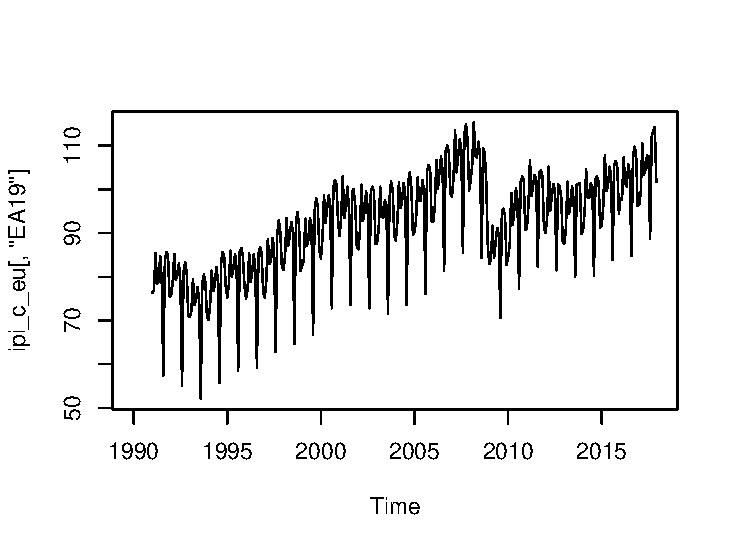
\includegraphics{img/img-basic_raw_data_plot-1} \end{center}

\end{CodeChunk}

\hypertarget{print-styling}{%
\subsection{Print styling}\label{print-styling}}

By default, a color styling is used for the print methods of the objects
created by \pkg{RJDemetra}. It can causes troubles with some outputs
(for example with \pkg{rmarkdown} \citep{rmarkdown}) and can be disabled
in each print function with the argument
\code{enable_print_style = FALSE} or setting the global option
\code{enable_print_style}:

\begin{CodeChunk}

\begin{CodeInput}
R> options(enable_print_style = FALSE)
\end{CodeInput}
\end{CodeChunk}

\hypertarget{pre-def-est}{%
\section{Estimate a pre-defined RegARIMA and SA
model}\label{pre-def-est}}

As in JDemetra+, the \pkg{RJDemetra} package allows to perform seasonal
adjustment using pre-defined model specifications. The pre-defined
specifications correspond to most commonly used specifications and users
are recommended to start their analysis with one of them. They are
separately defined for TRAMO-SEATS and X-13ARIMA-SEATS estimation
methods. It is also possible to perform only the first step of seasonal
adjustment (the RegARIMA estimation). The pre-defined model
specifications are described in tables \ref{tab:pre_def_ts} and
\ref{tab:pre_def_x13}. They are identical for pre-adjustment (column 1)
and for seasonal adjustment (column 2). With more details, setting
described in tables tables \ref{tab:pre_def_ts} and
\ref{tab:pre_def_x13} are:

\begin{itemize}
\tightlist
\item
  Transformation test: a test to choose between an additive
  decomposition (no transformation) and a multiplicative decomposition
  (logarithmic transformation).\\
\item
  Pre-adjustment for leap-year: in the case of a multiplicaive
  decomposition; a correction of the February values is applied to the
  original series (before transformation). The original values in
  February are multiplied by \(\frac{28.25}{29}\) for leap years, by
  \(\frac{28.25}{28}\) for non-leap years and values for other months
  are not modified. In the case of multiplicative models, this is
  equivalent to adding a leap year regressor
  \citep{bell1992lengthmonthadj}.
\item
  Working days: a pre-test is made for a presence of a working day
  effect.\\
\item
  Trading days: a pre-test is made for a presence of a trading day
  effect.\\
\item
  Easter: a pre-test for a presence of the Easter effect. The default
  length of the Easter effect is 6 days (for TRAMO-SEATS specifications)
  and 8 days (for X-13ARIMA-SEATS specifications).\\
\item
  Outliers: an automatic identification of three types of outliers: AO
  (additive outliers), LS (level shifts) and TC (transitory changes),
  using a default critical value.\\
\item
  ARIMA model: the choice between fixing the ARIMA model structure to
  (0,1,1)(0,1,1) (Airlin model) or searching for the ARIMA model using
  an automatic model identification procedure. The Airline model is used
  as a default model in several TRAMO-SEATS+ and X-13ARIMA-SEATS
  specifications because it has been shown in many studies that this
  model is appropriate for many real seasonal monthly or a quarterly
  time series. Moreover, the Airline model approximates well many other
  models and provides an excellent ``benchmark'' model
  \citep{maravall2009identification}.
\end{itemize}

\begin{table}[t]

\caption{\label{tab:pre_def_ts}Pre-defined specification for TRAMO and TRAMO-SEATS}
\centering
\fontsize{7}{9}\selectfont
\begin{tabular}{c>{\centering\arraybackslash}p{1.cm}>{\centering\arraybackslash}p{1.cm}>{\centering\arraybackslash}p{1.5cm}>{\centering\arraybackslash}p{0.9cm}>{\centering\arraybackslash}p{0.9cm}>{\centering\arraybackslash}p{1.5cm}>{\centering\arraybackslash}p{0.9cm}c}
\toprule
\multicolumn{2}{c}{Specification} & \multicolumn{1}{c}{} \\
\cmidrule(l{3pt}r{3pt}){1-2}
TRAMO & TRAMO-SEATS & Trans-formation & Pre-adjust-ment for leap-year & Working days & Trading days & Easter effect & Outliers & ARIMA model\\
\midrule
TR0 & RSA0 & no & no & no & no & no & no & (0,1,1)(0,1,1)\\
TR1 & RSA1 & test & no & no & no & no & test & (0,1,1)(0,1,1)\\
TR2 & RSA2 & test & no & test & no & test & test & (0,1,1)(0,1,1)\\
TR3 & RSA3 & test & no & no & no & no & test & AMI\\
TR4 & RSA4 & test & no & test & no & test & test & AMI\\
\addlinespace
TR5 & RSA5 & test & no & no & yes & test (Standard) & test & AMI\\
TRfull (default) & RSAfull (default) & test & yes & no & test & test (Include Easter) & test & AMI\\
\bottomrule
\end{tabular}
\end{table}

\begin{table}[t]

\caption{\label{tab:pre_def_x13}Pre-defined specification for RegARIMA and X-13ARIMA-SEATS}
\centering
\fontsize{7}{9}\selectfont
\begin{tabular}{c>{\centering\arraybackslash}p{1.7cm}>{\centering\arraybackslash}p{1.cm}>{\centering\arraybackslash}p{1.4cm}>{\centering\arraybackslash}p{0.9cm}>{\centering\arraybackslash}p{0.9cm}>{\centering\arraybackslash}p{0.9cm}>{\centering\arraybackslash}p{0.9cm}c}
\toprule
\multicolumn{2}{c}{Specification} & \multicolumn{1}{c}{} \\
\cmidrule(l{3pt}r{3pt}){1-2}
RegARIMA & X-13ARIMA-SEATS & Trans-formation & Pre-adjust-ment for leap-year & Working days & Trading days & Easter effect & Outliers & ARIMA model\\
\midrule
RG0 &  & no & no & no & no & no & no & (0,1,1)(0,1,1)\\
RG1 & RSA1 & test & no & no & no & no & test & (0,1,1)(0,1,1)\\
RG2c & RSA2c & test & test & test & no & test & test & (0,1,1)(0,1,1)\\
RG3 & RSA3 & test & no & no & no & no & test & AMI\\
RG4c & RSA4c & test & test & test & no & test & test & AMI\\
\addlinespace
RG5c (default) & RSA5 (default) & test & test & no & test & test & test & AMI\\
\bottomrule
\end{tabular}
\end{table}

Four functions can be used in \pkg{RJDemetra} to perform an estimation
with the pre-defined specification:

\begin{itemize}
\tightlist
\item
  RegARIMA

  \begin{itemize}
  \tightlist
  \item
    X-13ARIMA method: \code{regarima_def_x13()}
  \item
    TRAMO-SEATS method: \code{regarima_def_tramoseats()}
  \end{itemize}
\item
  Seasonal adjustment

  \begin{itemize}
  \tightlist
  \item
    X-13ARIMA method: \code{x13_def()}
  \item
    TRAMO-SEATS method: \code{tramoseats_def()}
  \end{itemize}
\end{itemize}

For examples:

\begin{CodeChunk}

\begin{CodeInput}
R> myseries <- ipi_c_eu[, "EA19"]
R> 
R> regx13 <- regarima_def_x13(myseries, spec = "RG5c")
R> regts <- regarima_def_tramoseats(myseries, spec = "TRfull")
R> sax13 <- x13_def(myseries, spec = "RSA3", userdefined = NULL)
R> sats <- tramoseats_def(myseries, spec = "RSAfull", userdefined = NULL)
\end{CodeInput}
\end{CodeChunk}

In section \ref{user-def-spec} it is presented how to modify model
specifications, including the possibility to incorprate user-defined
regressors.

\hypertarget{sa-object-structure}{%
\section{SA object structure}\label{sa-object-structure}}

In the previous section it was presented how to run a RegARIMA and
complete seasonal adjustment estimation with pre-defined model
specifications. In this section the outcome will be described in detail.

As a result of seasonal adjustment estimation (e.g.~function
\code {x13_def} or \code {tramoseats_def}) a S3 class object
(\code{sa_object}) is created. It has a class \code{c("SA","X13")} or
\code{c("SA","TRAMO_SEATS")} depending on the used estimation method.
The \code{sa_object} consits of lists of S3 class sub-objects. For each
of the class \code{print, plot} methods are defined. The complete
structure of the \code{sa_object} is presented in table
\ref{tab:obj_tab}. The first column gives the name of \code{sa_object}
sub-components, the second the level of the sub-components, the third
their type, and the fourth and fifth the name of the new created S3
classe (if any). Where the forth column corresponds to the case when the
estimation is done with X-12ARIMA/X-13ARIMA and fifth when estimated
with TRAMO-SEATS+. In general, the \code{sa_object} contains the
following five objects: \textbf{regarima}, \textbf{decomposition},
\textbf{final}, \textbf{diagnostics} and \textbf{user\_defined}.
Independently which of the two methods is used the regarima, final and
diagnostics objects contain the same components, though with different
classes (see column 4 and 5). Whereas, the object decomposition differs
for the two methods. The object user\_defined is empty unless additional
output was requested by the user (see next sub-sections). Finally, when
estimating RegARIMA only the regarima object is created.

\begingroup\fontsize{7}{9}\selectfont

\begin{longtable}{lllll}
\caption{\label{tab:unnamed-chunk-6}\label{tab:obj_tab}SA object structure}\\
\toprule
\multicolumn{1}{c}{ } & \multicolumn{1}{c}{ } & \multicolumn{1}{c}{ } & \multicolumn{2}{c}{When adjusted with:} \\
\cmidrule(l{3pt}r{3pt}){4-5}
\multicolumn{1}{c}{\em{ }} & \multicolumn{1}{c}{\em{ }} & \multicolumn{1}{c}{\em{ }} & \multicolumn{1}{c}{\em{x13/x13\_def}} & \multicolumn{1}{c}{\em{ tramoseats/tramoseats\_def}} \\
\cmidrule(l{3pt}r{3pt}){4-4} \cmidrule(l{3pt}r{3pt}){5-5}
Object & Level & Type & Class & Class\\
\midrule
sa\_object & 0 & list & SA, X13 & SA, TRAMO\_SEATS\\
\textbf{\hspace{1em}regarima} & \textbf{1} & \textbf{list} & \textbf{regarima, X13} & \textbf{regarima, TRAMO\_SEATS}\\
\hspace{2em}specification & 2 & list &  & \\
\hspace{3em}estimate & 3 & data.frame &  & \\
\hspace{3em}transform & 3 & data.frame &  & \\
\addlinespace
\hspace{3em}regression & 3 & list &  & \\
\hspace{4em}userdef & 4 & list &  & \\
\hspace{5em}specification & 5 & data.frame &  & \\
\hspace{5em}outliers & 5 & data.frame or NA(empty) &  & \\
\hspace{5em}variables & 5 & list &  & \\
\addlinespace
\hspace{6em}series & 6 & mts, ts, matrix or NA(empty) &  & \\
\hspace{6em}description & 6 & data.frame or NA(empty) &  & \\
\hspace{4em}trading.days & 4 & data.frame &  & \\
\hspace{4em}easter & 4 & data.frame &  & \\
\hspace{3em}outliers & 3 & data.frame &  & \\
\addlinespace
\hspace{3em}arima & 3 & list &  & \\
\hspace{4em}specification & 4 & data.frame &  & \\
\hspace{4em}coefficients & 4 & data.frame or NA(empty) &  & \\
\hspace{3em}forecast & 3 & data.frame &  & \\
\hspace{3em}span & 3 & data.frame &  & \\
\addlinespace
\hspace{2em}arma & 2 & vector - numeric &  & \\
\hspace{2em}arima.coefficients & 2 & matrix &  & \\
\hspace{2em}regression.coefficients & 2 & matrix &  & \\
\hspace{2em}loglik & 2 & matrix &  & \\
\hspace{2em}model & 2 & list &  \vphantom{1} & \\
\addlinespace
\hspace{3em}spec\_rslt & 3 & data.frame &  & \\
\hspace{3em}effects & 3 & mts, ts, matrix &  & \\
\hspace{2em}residuals & 2 & ts &  & \\
\hspace{2em}residuals.stat & 2 & list &  & \\
\hspace{3em}st.error & 3 & numeric &  & \\
\addlinespace
\hspace{3em}tests & 3 & data.frame & regarima\_rtests, data.frame & \\
\hspace{2em}forecast & 2 & mts, ts, matrix &  & \\
\textbf{\hspace{1em}decomposition} & \textbf{1} & \textbf{list} & \textbf{decomposition\_X11} & \textbf{}\\
\hspace{2em}specification & 2 & data.frame & X11\_spec, data.frame & \\
\hspace{2em}mode & 2 & character &  \vphantom{1} & \\
\addlinespace
\hspace{2em}mstats & 2 & matrix &  & \\
\hspace{2em}si\_ratio & 2 & mts, ts, matrix &  & \\
\hspace{2em}s\_filter & 2 & vector - character &  & \\
\hspace{2em}t\_filter & 2 & character &  & \\
\textbf{\hspace{1em}decomposition} & \textbf{1} & \textbf{list} & \textbf{} & \textbf{decomposition\_SEATS}\\
\addlinespace
\hspace{2em}specification & 2 & data.frame & seats\_spec, data.frame & \\
\hspace{2em}mode & 2 & character &  & \\
\hspace{2em}model & 2 & list &  & \\
\hspace{3em}model & 3 & matrix or empty list &  & \\
\hspace{3em}sa & 3 & matrix or empty list &  & \\
\addlinespace
\hspace{3em}trend & 3 & matrix or empty list &  & \\
\hspace{3em}seasonal & 3 & matrix or empty list &  & \\
\hspace{3em}transitory & 3 & matrix or empty list &  & \\
\hspace{3em}irregular & 3 & matrix or empty list &  & \\
\hspace{2em}linearized & 2 & mts, ts, matrix &  & \\
\addlinespace
\hspace{2em}components & 2 & mts, ts, matrix &  & \\
\textbf{\hspace{1em}final} & \textbf{1} & \textbf{list} & \textbf{final} & \textbf{}\\
\hspace{2em}series & 2 & mts, ts, matrix &  & \\
\hspace{2em}forecasts & 2 & mts, ts, matrix &  & \\
\textbf{\hspace{1em}diagnostics} & \textbf{1} & \textbf{list} & \textbf{diagnostics} & \textbf{}\\
\addlinespace
\hspace{2em}variance\_decomposition & 2 & data.frame &  & \\
\hspace{2em}combined\_test & 2 & list & combined\_test & \\
\hspace{3em}tests\_for\_stable\_seasonality & 3 & data.frame &  & \\
\hspace{3em}combined\_seasonality\_test & 3 & character &  & \\
\hspace{2em}residuals\_test & 2 & data.frame &  & \\
\addlinespace
\textbf{\hspace{1em}user\_defined} & \textbf{1} & \textbf{list} & \textbf{user\_defined} & \textbf{}\\
\bottomrule
\end{longtable}
\endgroup{}

\hypertarget{regarima}{%
\subsection{Regarima}\label{regarima}}

Here we can also present the output: print and graphs.

\begin{CodeChunk}

\begin{CodeInput}
R> library(RJDemetra)
R> myseries <- ipi_c_eu[, "EA19"]
R> sax13 <- x13_def(myseries, spec = "RSA5c", userdefined = NULL)
R> sats <- tramoseats_def(myseries, spec = "RSAfull", userdefined = NULL)
R> ## PRINT THE RESULTS:
R> sax13$regarima
\end{CodeInput}

\begin{CodeOutput}
y = regression model + arima (1, 1, 2, 0, 1, 1)
Log-transformation: no
Coefficients:
          Estimate Std. Error
Phi(1)     -0.7695      0.117
Theta(1)   -1.0644      0.119
Theta(2)    0.3331      0.056
BTheta(1)  -0.5263      0.051

             Estimate Std. Error
Monday       -0.27760      0.103
Tuesday       0.01418      0.102
Wednesday     0.29139      0.103
Thursday     -0.36725      0.102
Friday        0.12606      0.102
Saturday      0.36548      0.103
Leap year     0.24961      0.316
AO (1-2016)   3.58591      0.837
TC (9-2008)  26.20114      3.037
LS (9-2008) -19.99432      2.470
AO (9-2008)  -6.10726      1.458


Residual standard error: 1.125 on 311 degrees of freedom
Log likelihood = -479.9, aic = 991.8 aicc = 993.7, bic(corrected for length) = 0.5122
\end{CodeOutput}

\begin{CodeInput}
R> ## PLOT THE RESULTS:
R> #plot(sax13$regarima)
\end{CodeInput}
\end{CodeChunk}

\hypertarget{decomposition}{%
\subsection{Decomposition}\label{decomposition}}

\hypertarget{final}{%
\subsection{Final}\label{final}}

\hypertarget{diagnostics}{%
\subsection{Diagnostics}\label{diagnostics}}

\hypertarget{user-defined}{%
\subsection{user defined}\label{user-defined}}

\hypertarget{user-def-spec}{%
\section{Model specification: creation and
modification}\label{user-def-spec}}

\hypertarget{x13}{%
\subsection{X13}\label{x13}}

\hypertarget{tramoseats}{%
\subsection{TRAMOSEATS}\label{tramoseats}}

\hypertarget{regarima-1}{%
\subsection{Regarima}\label{regarima-1}}

\hypertarget{wrong-specifications-corrections}{%
\subsection{Wrong specifications
corrections}\label{wrong-specifications-corrections}}

Parler des corrections automatiques ?

\hypertarget{manipulate-workspace}{%
\section{Manipulate JDemetra+ workspaces}\label{manipulate-workspace}}

\pkg{RJDemetra} allows to interact with JDemetra+ workspace that can be
openned by the software. A workspace includes :

\begin{itemize}
\tightlist
\item
  The XML file that enables the user to import the workspace to
  JDemetra+ and to display it content;\\
\item
  A folder containing several sub-folfders that correspond to the
  different types of items created by the user.
\end{itemize}

Each workspace can contain several multi-processings and each
multi-processing stores the results of the seasonal adjustment procedure
performed with the TRAMO-SEATS or X-13ARIMA-SEATS methods.

Export models to workspace allows to store easily the seasonal
adjustment models, to change the specifications with the JDemetra+
graphical interface and to give models to non R users (à reformuler).

\hypertarget{export-wk}{%
\subsection{Export a workspace}\label{export-wk}}

Four functions have to be used to export models:

\begin{itemize}
\tightlist
\item
  \code{new_workspace()} to create a workspace;\\
\item
  \code{new_multiprocessing()} to create a multi-processing in a
  workspace;\\
\item
  \code{add_sa_item()} to add a seasonal adjustment model to a
  multi-processing;\\
\item
  \code{save_workspace()} to export the workspace.
\end{itemize}

The following command export the seasonal adjustment models compute by
TRAMO-SEATS+ and X-13ARIMA-SEATS:

\begin{CodeChunk}

\begin{CodeInput}
R> myseries <- ipi_c_eu[, "EA19"]
R> sa_x13 <- x13_def(myseries)
R> sa_ts <- tramoseats_def(myseries)
\end{CodeInput}
\end{CodeChunk}

To create a workspace and a multi-processing names ``MP-1'':

\begin{CodeChunk}

\begin{CodeInput}
R> wk <- new_workspace()
R> new_multiprocessing(wk, name = "MP-1")
\end{CodeInput}
\end{CodeChunk}

The two models will be added in the multiprocessing ``MP1'': the name of
the seasonal adjustment model computed with X-13ARIMA-SEATS will be ``SA
with X13'' and the one with TRAMO-SEATS+ will be ``SA with TramoSeats''.

\begin{CodeChunk}

\begin{CodeInput}
R> add_sa_item(wk, multiprocessing = "MP-1",
R+             sa_obj = sa_x13, name =  "SA with X13")
R> add_sa_item(wk, multiprocessing =  "MP-1",
R+             sa_obj = sa_ts, name = "SA with TramoSeats")
\end{CodeInput}
\end{CodeChunk}

The workspace exported is named ``workspace.xml'':

\begin{CodeChunk}

\begin{CodeInput}
R> save_workspace(wk, file =  "workspace.xml")
\end{CodeInput}
\end{CodeChunk}

\hypertarget{import-a-workspace}{%
\subsection{Import a workspace}\label{import-a-workspace}}

Height functions can be used to import a workspace:

\begin{itemize}
\tightlist
\item
  \code{load_workspace()} to load a workspace;\\
\item
  \code{compute()} to compute the multi-processings: by default a
  workspace only contains definitions, computation is needed to get the
  seasonal adjustment model;\\
\item
  \code{get_model()} to get the seasonal adjusted models;\\
\item
  \code{get_ts()} to get the input raw time series, \code{get_object()}
  and \code{get_all_objects} to navigate inside the workspace (extract a
  multi-processing or a seasonal adjustment model), \code{get_name()} to
  get the names of the multiprocessings or the seasonal adjustment
  models and \code{count()} to count the number of multiprocessing or
  seasonal adjustment models.
\end{itemize}

For instance, to import the workspace created in section \ref{export-wk}
and to get the first multiprocessing and the first seasonal adjustment
model:

\begin{CodeChunk}

\begin{CodeInput}
R> wk <- load_workspace(file =  "workspace.xml")
R> mp1 <- get_object(wk, 1)
R> sa_item1 <- get_object(mp1, 1)
\end{CodeInput}
\end{CodeChunk}

To get the number of seasonal adjustment models in the multiprocessing:

\begin{CodeChunk}

\begin{CodeInput}
R> count(mp1)
\end{CodeInput}

\begin{CodeOutput}
[1] 2
\end{CodeOutput}
\end{CodeChunk}

And the name of the first seasonal adjustment model in JDemetra+:

\begin{CodeChunk}

\begin{CodeInput}
R> get_name(sa_item1) 
\end{CodeInput}

\begin{CodeOutput}
[1] "SA with X13"
\end{CodeOutput}
\end{CodeChunk}

Raw time series and seasonal adjustment model can now be imported:

\begin{CodeChunk}

\begin{CodeInput}
R> raw_ts <- get_ts(sa_item1)
R> compute(wk)
R> sa_model1 <- get_model(sa_item1, workspace = wk)
\end{CodeInput}
\end{CodeChunk}

\code{get_ts()} and \code{get_model()} can also be used directly to the
workspace or a multiprocessing to import all the raw time series or all
the seasonal adjustment model:

\begin{itemize}
\tightlist
\item
  for a multiprocessing the result is a list which each element contains
  the information of a seasonal adjustment model;\\
\item
  for a workspace the result is a list of length the number of
  multi-processing and which each element contains a list with the
  information of each seasonal adjustment model.
\end{itemize}

For example to get all raw time series of the workspace and all seasonal
adjustmen models of the first multi-processing:

\begin{CodeChunk}

\begin{CodeInput}
R> all_raw_ts <- get_ts(wk)
R> sa_models_of_mp1 <- get_model(mp1, workspace = wk)
\end{CodeInput}
\end{CodeChunk}

The imports of seasonal adjustment models from a workspace works well
when it has been created throw \pkg{RJDemetra}. They may be some
troubles when importing a workspace created with JDemetra+, in
particular:

\begin{itemize}
\tightlist
\item
  \pkg{RJDemetra} doesn't support yet user-defined calendars. A seasonal
  adjustment model defined with a specific calendar or user-defined
  calendar regressors will be partially imported. The result will be
  correct but changing the specification (throw \code{x13_spec()} or
  \code{tramoseats_spec()}) will erase user-defined calendars.\\
\item
  Seasonal adjustment models with ramp effect or intervention variables
  will be partially imported: the result of the imported model will be
  correct but changing the specification (throw \code{x13_spec()} or
  \code{tramoseats_spec()}) will erase them.\\
\item
  Seasonal adjustment models with no pre-processing (X-11 specification)
  are not supported: \code{NULL} object will be returned.
\end{itemize}

\hypertarget{advanced-usage-and-examples}{%
\section{Advanced usage and
examples}\label{advanced-usage-and-examples}}

\hypertarget{conclusion}{%
\section{Conclusion}\label{conclusion}}

\hypertarget{acknowledgments}{%
\section*{Acknowledgments}\label{acknowledgments}}
\addcontentsline{toc}{section}{Acknowledgments}

\renewcommand\refname{References}
\bibliography{biblio.bib}


\end{document}

